% Drawing 146/01-5 -- folder 146, batch 01, archive page 19 (PDF page 20).
% Transcription: une page entière de dessin, au crayon : un cylindre vertical dont le cercle supérieur est marqué $V_{\mathbb{C}}^{\omega}$, le cercle inférieur $V_{\mathbb{C}}^{\omega'}$, et le cercle médian (l'équateur) $V^{\omega}$, chacun avec une flèche de sens de rotation. Sur le cercle supérieur, les points $\tilde P_{a_1}^{\omega}$, $\tilde P_s^{\omega}$, $\tilde P_a^{\omega}$, et l'arc $\tilde d_s^{\omega}$ (un premier libellé biffé) tracé en gras de $\tilde P_{a_1}^{\omega}$ à $\tilde P_a^{\omega}$ ; de $\tilde P_a^{\omega}$ descend en gras un segment vertical, libellé $\tilde c_r$ ou $\tilde c_a^{\omega}$, jusqu'au point $\tilde Q_a$ de l'équateur ; le long de la verticale en pointillé issue de $\tilde P_{a_1}^{\omega}$ on lit $\tilde c_{a_1}^{\omega} = \tilde c_{\omega^{-1}(r_1)}$, et plus bas $\tilde c_{r_1} = \tilde c_{a_1}^{\omega'}$. Sur l'équateur, quatre petits cercles fléchés autour de points marqués (des lacets autour des points enlevés), les points $\tilde Q_{a_1}$, $\tilde R_{r_1}$, $\tilde R_s$, $R_r$, $\tilde Q_a$, les arcs $\tilde b_{r_1}$, $\tilde b_r$ (en gras), et un demi-cercle gras $\tilde a_r$ autour de $\tilde R_s$ ; un triangle hachuré à l'intérieur porte les libellés $r$, $r'$, $r''$, $r_1$, $r_2$, plusieurs autres étant biffés. Sur le cercle inférieur, les points $\tilde P_{a_1}^{\omega'}$, $\tilde P_s^{\omega}$, $\tilde P_a^{\omega'}$, les libellés $(\tilde d_{r_1})$, $\tilde d_{r_1}$ ou $\tilde d_s^{\omega'}$, et l'arc fléché $\tilde b_r^{\omega'}$. Des lettres pâles $a_\omega$, $a$, $a_{\omega'}$ dans la marge gauche du cylindre.
% Kind: surface figure (cylinder with marked points, paths and loops). Method 2 (schematic redraw from the facsimile). Status: partial.
% Notes: Skeleton redrawn: three circles of the cylinder (back halves drawn as the front, solid), sides, the dotted verticals, the bold path P~a1 -> P~a -> Q~a, the bold half-circle a~r around R~s, five looped points on the equator (the transcription says four; five are visible: two left, two right, one at the back), the hatched triangle and the hatched sliver on the left (approximate). Omitted: struck labels, the heavily overwritten labels by the hatched triangle (only r, r1, r'' kept), the pale letters a_omega, a, a_omega' left of the cylinder, the loose rotation arrows except the one by V_C^omega. Labels placed from the transcription, not re-read.
% Coordinates: 1 unit = 1 mm = 1/100 of the crop width (bbox in page fractions: [0.27, 0.18, 0.9, 0.74]).
% Redrawn by Claude (claude-opus-5-5), issue #73 pilot, 2026-11-07; not checked by a human; not compiled (no TeX in the session).
% Rights: reproduces part of the work -- behind RENDER_TRANSCRIPTS, never published by itself.
\documentclass[tikz,border=3pt]{standalone}
\usepackage{amsmath,amssymb}
\usetikzlibrary{patterns,arrows.meta}
\tikzset{pencil/.style={black!45}, struck/.style={black!35}, mark/.style={circle,draw,inner sep=1.3pt}, pt/.style={circle,fill,inner sep=0.9pt}, opt/.style={circle,draw,fill=white,inner sep=1.1pt}}
\begin{document}
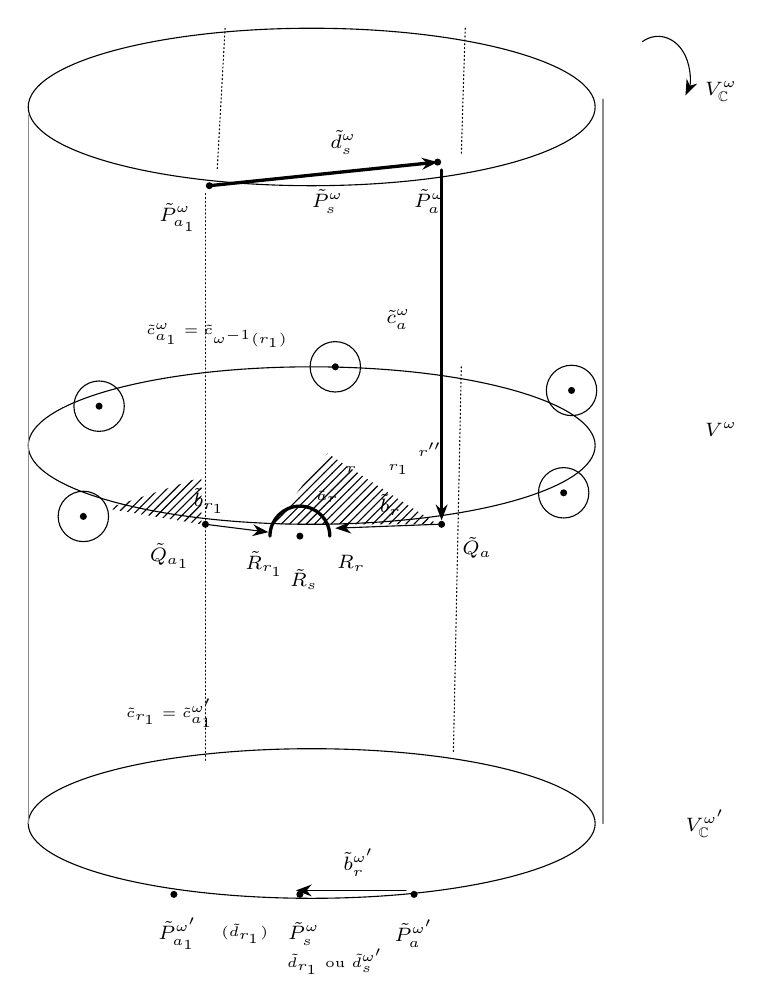
\begin{tikzpicture}[x=1mm,y=1mm,line cap=round,line join=round,font=\scriptsize]
\draw (42,-16) ellipse[x radius=36, y radius=10];
\draw (42,-59) ellipse[x radius=36, y radius=10];
\draw (42,-107) ellipse[x radius=36, y radius=9.5];
\draw[pencil] (6,-17) -- (6,-107);
\draw[pencil] (79,-15) -- (79,-107);
\draw[densely dotted] (31,-6) -- (30,-24);
\draw[densely dotted] (61.5,-6) -- (61,-22);
\draw[densely dotted] (28.5,-27) -- (28.5,-99);
\draw[densely dotted] (61,-49) -- (60,-98);
\draw[very thick,-{Stealth[length=2mm]}] (29,-26) -- (58,-23);
\draw[very thick,-{Stealth[length=2mm]}] (58.5,-24) -- (58.5,-68.5);
\draw[very thick] (44.3,-70.5) arc[start angle=0, end angle=180, x radius=3.8, y radius=3.8];
\node[pt] at (40.5,-70.5) {};
\draw[-{Stealth[length=2mm]}] (58,-69) -- (45,-69.5);
\draw[-{Stealth[length=2mm]}] (28.5,-69) -- (36.5,-70);
\draw (15,-54) circle[radius=3.2];
\draw (13,-68) circle[radius=3.2];
\draw (75,-52) circle[radius=3.2];
\draw (74,-65) circle[radius=3.2];
\draw (45,-49) circle[radius=3.2];
\node[pt] at (15,-54) {};
\node[pt] at (13,-68) {};
\node[pt] at (75,-52) {};
\node[pt] at (74,-65) {};
\node[pt] at (45,-49) {};
\node[pt] at (29,-26) {};
\node[pt] at (58,-23) {};
\node[pt] at (28.5,-69) {};
\node[pt] at (58.5,-69) {};
\fill[pattern=north east lines] (37,-69) -- (44,-60) -- (58,-69) -- cycle;
\fill[pattern=north east lines] (16,-67) -- (28,-63) -- (28,-69) -- cycle;
\draw[-{Stealth[length=2mm]}] (84,-7.7) arc[start angle=120, end angle=-30, x radius=4, y radius=5];
\node[inner sep=1pt] at (94,-14) {\scriptsize $V_{\mathbb{C}}^{\omega}$};
\node[inner sep=1pt] at (94,-57) {\scriptsize $V^{\omega}$};
\node[inner sep=1pt] at (92,-107) {\scriptsize $V_{\mathbb{C}}^{\omega'}$};
\node[inner sep=1pt] at (25,-30) {\scriptsize $\tilde P_{a_1}^{\omega}$};
\node[inner sep=1pt] at (44,-28) {\scriptsize $\tilde P_s^{\omega}$};
\node[inner sep=1pt] at (57,-28) {\scriptsize $\tilde P_a^{\omega}$};
\node[inner sep=1pt] at (46,-20.5) {\scriptsize $\tilde d_s^{\omega}$};
\node[inner sep=1pt] at (53,-43) {\scriptsize $\tilde c_a^{\omega}$};
\node[inner sep=1pt] at (30,-45) {\tiny $\tilde c_{a_1}^{\omega}=\tilde c_{\omega^{-1}(r_1)}$};
\node[inner sep=1pt] at (24,-73) {\scriptsize $\tilde Q_{a_1}$};
\node[inner sep=1pt] at (36,-74) {\scriptsize $\tilde R_{r_1}$};
\node[inner sep=1pt] at (41,-76) {\scriptsize $\tilde R_s$};
\node[inner sep=1pt] at (47,-74) {\scriptsize $R_r$};
\node[inner sep=1pt] at (63,-72) {\scriptsize $\tilde Q_a$};
\node[inner sep=1pt] at (29,-66) {\scriptsize $\tilde b_{r_1}$};
\node[inner sep=1pt] at (52,-66.5) {\scriptsize $\tilde b_r$};
\node[inner sep=1pt] at (44,-65.5) {\tiny $\tilde a_r$};
\node[inner sep=1pt] at (47,-62) {\tiny $r$};
\node[inner sep=1pt] at (53,-62) {\tiny $r_1$};
\node[inner sep=1pt] at (57,-59.5) {\tiny $r''$};
\node[inner sep=1pt] at (24,-93) {\tiny $\tilde c_{r_1}=\tilde c_{a_1}^{\omega'}$};
\draw[-{Stealth[length=2mm]}] (54,-115.5) -- (40,-115.5);
\node[inner sep=1pt] at (48,-112) {\scriptsize $\tilde b_r^{\omega'}$};
\node[inner sep=1pt] at (25,-121) {\scriptsize $\tilde P_{a_1}^{\omega'}$};
\node[inner sep=1pt] at (33.5,-121) {\tiny $(\tilde d_{r_1})$};
\node[inner sep=1pt] at (41,-121) {\scriptsize $\tilde P_s^{\omega}$};
\node[inner sep=1pt] at (55,-121) {\scriptsize $\tilde P_a^{\omega'}$};
\node[inner sep=1pt] at (45,-124.5) {\tiny $\tilde d_{r_1}$ ou $\tilde d_s^{\omega'}$};
\node[pt] at (24.5,-116) {};
\node[pt] at (40.5,-116) {};
\node[pt] at (55,-116) {};
\end{tikzpicture}
\end{document}
